\documentclass[thesis.tex]{subfiles}

\begin{document}

\chapter{Prerequisites and Related Work}  \label{chap:preqAndRel}

This chapter lists and describes the necessary topics to follow this thesis. It explains SCION's structure, functionality and details about the component as for example the border router. SCIONLab itself and its work is also outlined. At last, a short description about Prometheus and its used features will be given to understand how the experiment was done.
The second part of the chapter will list related works which tried to solve the problem of multi path communication abuse by regulating or monitoring the behavior. The work on SIPRA and a VirtualCredit system will be presented, which are designed for SCION. Additional work for other types of networks will also be discussed.

\section{Prerequisites} \label{chap:preq}

\subsection{SCION} \cite{SCIONPaper, SCIONBook}

SCION, an acronym for \textbf{S}calability, \textbf{C}ontrol and \textbf{I}solation \textbf{O}n \textbf{N}ext-generation networks, provides a green-field solution for problems of the current Internet, which is named in this content as the \textit{legacy internet}. The main difference between them is \textit{path-transparency}. In the current existing IP routing protocol the end-hosts cannot chose a path, but must rely on the router between them to find a good path. This leads to the problem, that the receiver cannot verify, if the packets were modified nor if the taken path was trustworthy. SCION allows the end hosts to chose between communication paths and also to see the path of a packet on the end-host. The fundamental change needs a different organization of the network nodes, which will be described in this part.

\autoref{fig:prequirement:scionStructure} shows an example SCION network from \cite{SCIONPaper}. This topology consists of \textbf{Is}olation \textbf{D}omains (ISD) and each node of it is considered an \textbf{A}utonomous \textbf{S}ystem (AS). They represent exactly one physical end-host, a whole companies network or an \textbf{I}nternet \textbf{S}ervice \textbf{P}rovider (ISP)'s network. Each ISD is administered and initially created by a small group of ASes, which are referred to \textit{Core} ASes and forms the \textit{Core} of an ISD. They are responsible to define a policy which applies to all member of the ISD and is called the \textbf{T}rust \textbf{R}oot \textbf{C}onfiguration (TRC). Concluding this each ISD has its own rules to create connection and also defines the name the ISD. The Core ASes are also connect with other ISDs and link their ISDs to them. Additionally an AS can belong to multiple ISDs at one time, which is the case for the AS \textbf{H}.

An AS needs to know the path to another AS to communicate to them. This routing problem is solved with a process called \textit{beaconing}. A core AS announces such a beaconing inside its ISDs and learns the different paths from a core AS to a non-core AS. The ASes respond to this beaconing and over time the topology is created. On the other side, a non-core AS explores by beaconing the paths to the core-AS. The same procedure is done for inter-ISD communication by the core-ASes. The up-segment from a non-core AS to the Core and the down-segment from the beaconing of a core-AS are merged together and send to the \textit{path-server}. This component handles routing requests from one AS to another AS and responds with a set of possible paths to take. The elements of this set depend on the TRC of the ISD. For example, one ISD does not want to enable multiple path communication and only responds with the first available path.

One advantage of this structured routing is that a communication does not leave an ISD when it is not necessary. This enables to create ISDs for different security or efficiency scenarios. Packets are only routed in a trusted zone when they need to be. The legacy internet do not guarantee this behavior. A packet from OvGU-Magdeburg to ETH-Zuerich could be routed over different location in the world without control over it. If both of them were inside one ISD containing only research institutes, than the packet would be guaranteed to not leave this ISD because it is not necessary.

Another advantage is the possibility to choose an alternative way. This is interesting in cases a path segment has a failure and should be avoided for different reasons like malicious attacks or technical failures. The legacy internet relies on the Border-Gateway-Protocol (BGP) \cite{rekhter2005border, Halabi.1997}, when was inspected by many researcher for its fault-tolerance and stability. It was also shown in \cite{Sahoo.2006} that the reaction time (convergence) for realistic topologies takes seconds to minutes for the protocol to adjust to failures. A similar result was given by \cite{Labovitz.2001} of a delay of 3 minutes for 30\% the cases and even higher as 15 minutes in total. In SCION this slow reaction problem is minimized by letting the user choose different path. If one path is not responding the node can request for another path or use one of the provided alternatives.

The multiple paths to the target can also be used for a better bandwidth utilization. Instead of sending the data over only one link the stream can be split into multiple sub streams and transfered over the available paths to the target. 
This leads to a better utilized networks capacity because otherwise unused links are used and not idle. Bandwidth is cannot be saved or stored, it can only be used in a moment or it would be wasted. But this also can lead to an unwanted flood of the network and can create multiple congestions, unintentionally. This would negate the advantage and should only be used with caution. Because of the potential misuse of such a multipath communication several studies have been conducted which are explained in \autoref{chap:prevwork}

\begin{figure}
	\centering
	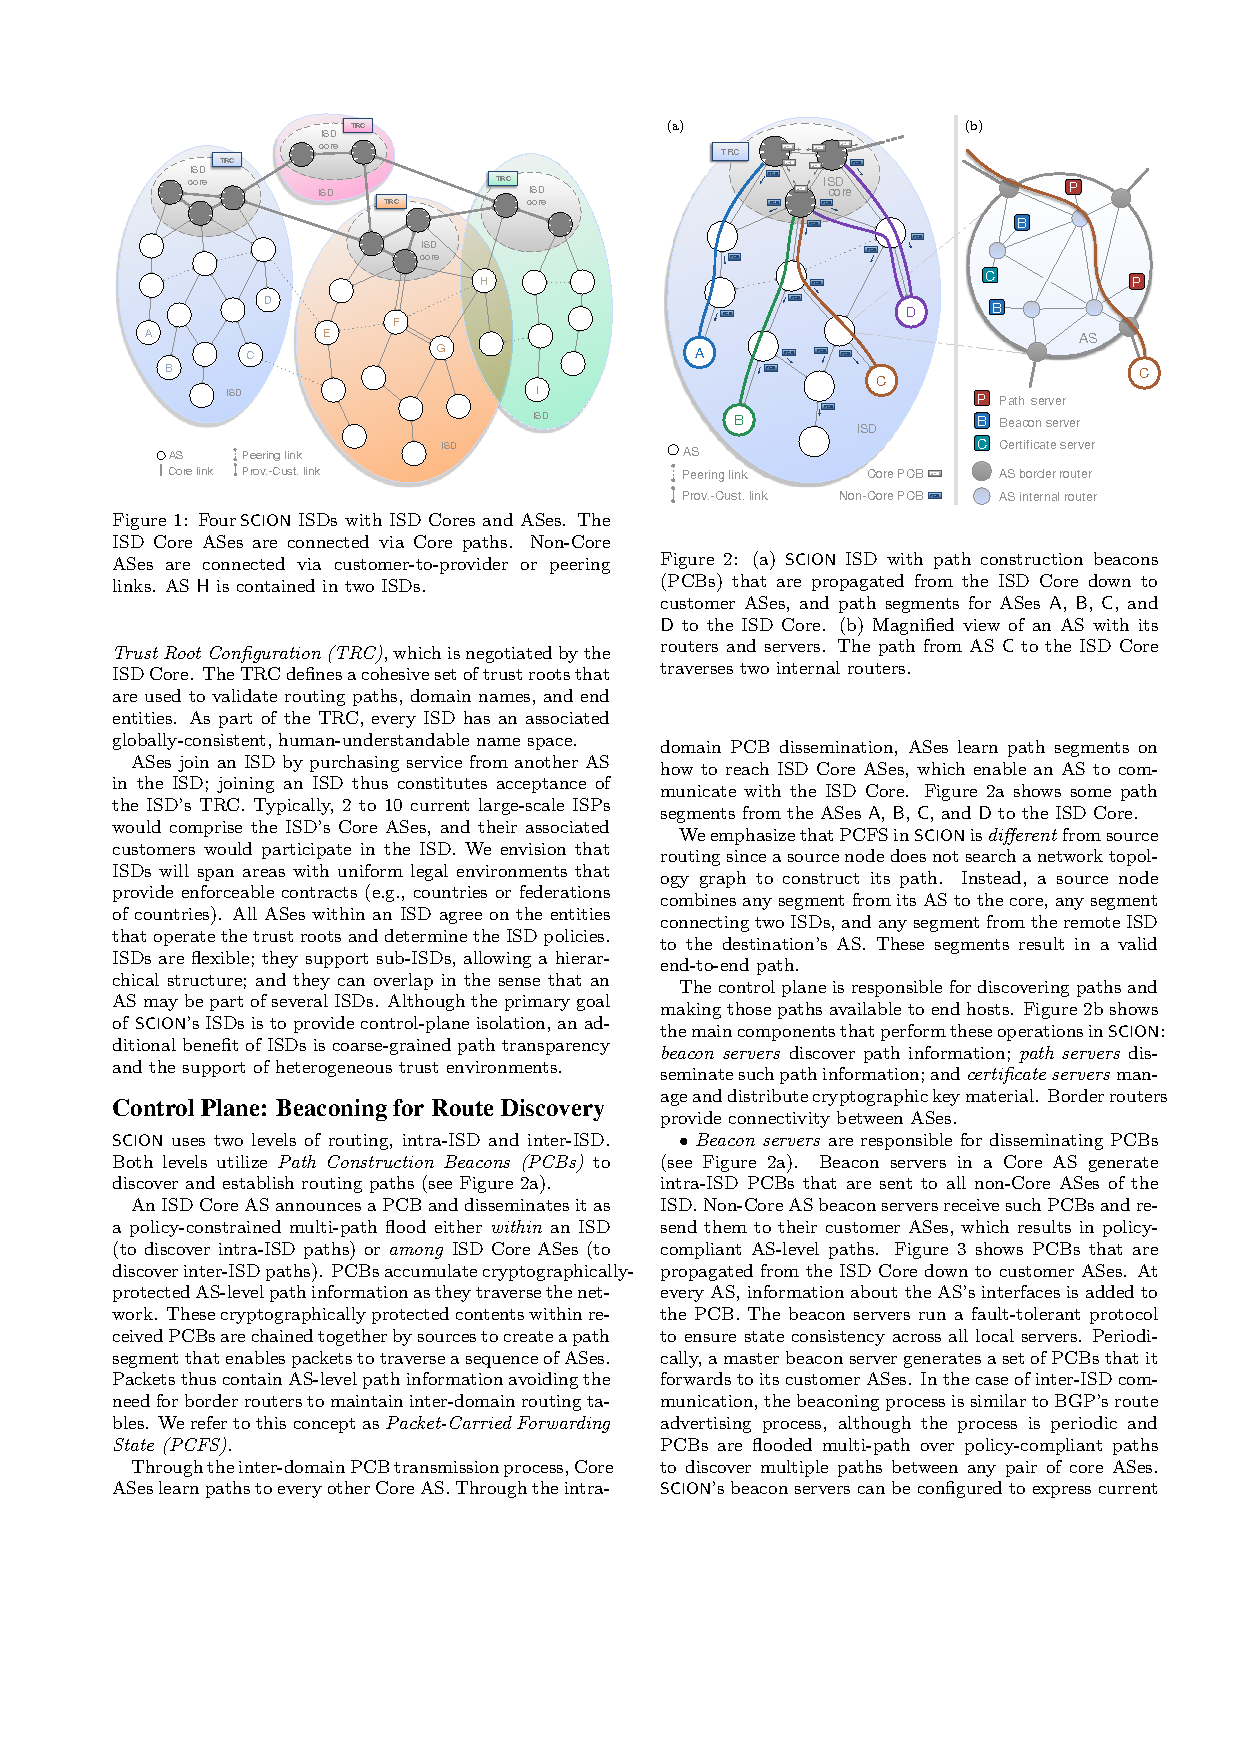
\includegraphics[trim=19mm 214mm 105mm 19mm ,clip,width=0.5\linewidth]{2015-SCION-short_3.pdf}
	\caption{Four SCION ISDs with ISD Cores and ASes \cite{SCIONPaper}}
	\label{fig:prequirement:scionStructure}
\end{figure}

\subsection{Prometheus} 

"Prometheus is an open-source systems monitoring and alerting toolkit [...]" \footnote{\url{https://prometheus.io/}, 18.04.2018}. This framework consisting of a \textit{Prometheus server} and an API to create and gather data about programs, which is implemented by the \textit{Prometheus clients}. Each client defines a data model of different \textit{metrics} to monitor. These metrics are collected by the Prometheus server in a given scrap interval and stored on the server side. A simple Web UI enables the user to write queries and analyze the data, for example extracting the maximum bandwidth at a given time.

The client API defines four different metric types. The \textit{counter} represents a data which can only go up while the \textit{gauge} can also go down over time. An example for a counter is the total bandwidth in bytes since the border router start while a gauge can be the current memory usage. The two other types are the \textit{histogram}, which samples observations in different buckets, and the \textit{summary} which does the same as a counter but also calculates quantiles over a sliding time window. Each metric consists of the value itself as a double-precision floating point number and a UTC time stamp. The client defines the type of the metric and the name and continually updates the value. The metrics are exported over an HTTP based API. The endpoint is typically {\lstinline|http://[HOST]:[PORT]/metrics|} which responds with a list of all metrics and their values at the time of request. The Prometheus client API was already implemented in the border router, the path, the beaconing and the certificate server. An example of this is seen in \autoref{app:promMetric}

\begin{easylist}
    \MyListProperties
    # SCION
    ## Origins of SCION
    ## Structure of SCION
    ## \textit{Figure example topology}
    ## Explain relevant components of an AS
    ### Path Server + Path Discovery
    ### Border Router
    ## SCIONLab
    ### Goal \& How it works
    ### Coordinator in ETH Zurich
    ## Multipath method
    ### How does it work
    ### \textit{Figure of example}
    ### Explanation of example
    ### Difference to legacy methods
    # Other prerequisites
\end{easylist}

\section{Related Work}\label{chap:prevwork}

\begin{easylist}
	\MyListProperties
	# SIBRA \cite{Basescu.2016}
	## General Idea
	## Why it partially solves the problem
	## Advantages
	## Explain why to complex for SCIONLab
	# Virtual Credit \cite{DennisMeyer.2017}
	## General Idea
	## Why it partially solves the problem
	## Advantages
	## Use the idea to define a greedy user (more credits = less greedy)
	# \cite{Zhu.2014}
	## General Idea
	## Use for this work
	# Prioritizing network traffic as a solution (QoP)
	## Why this is not enough 
	# Game Theory - Inspection game
	## General idea
	## Nash Equilibrium in mixed strategy
	## How this can be applied to this thesis (probability)
\end{easylist}

\subfilebib % Makes bibliography available when compiling as subfile
\end{document}